\documentclass[openany, a4paper]{book}

\usepackage{afterpage}
\usepackage{fontspec}
\usepackage{geometry}
\usepackage{hyperref}
\usepackage{lscape}
\usepackage{siunitx}
\usepackage{titling}

\newcommand*{\subtitle}[1]{\gdef\thesubtitle{#1}}

\title{CRAPS Kernel}
\subtitle{Final Report}
\author{
       Maxime Arthaud
  \and Korantin Auguste
  \and Martin Carton
  \and Étienne Lebrun
  \and Pierre-Louis Michel
}

\newcommand{\risk}[4]{%
  \noindent
  \begin{center}
    \begin{tabular}{|p{0.8\textwidth}|c|}
        \hline
        #2 & $#1$
      \\\hline
        \multicolumn{2}{|p{0.9\textwidth}|}{#3}
      \\\hline
        \multicolumn{2}{|p{0.9\textwidth}|}{#4}
      \\\hline
    \end{tabular}
  \end{center}
}

\begin{document}
  \begin{titlepage}
  \begin{center}
    
\includegraphics[height=1cm]{LogoEnseeiht}\\\vspace{1cm}
    \hrule\vspace{0.5cm}
    \textsc{\Large\thesubtitle}
    \\\vspace{0.5cm}

    \textbf{\huge\thetitle}
    \\\vspace{0.4cm}
    \hrule\vspace{2cm}

    {\large
      Maxime~\textsc{Arthaud}      \\
      Korantin~\textsc{Auguste}    \\
      Martin~\textsc{Carton}       \\
      Étienne~\textsc{Lebrun}
    }

    \vfill
    {\large January -- March 2015}
  \end{center}
\end{titlepage}


  \chapter*{Acknowledgments}
    We would like to thank Jean-Christophe Buisson for giving us all the tools
    related to CRAPS that he has developed. We won a lot of time thanks to this.

    \paragraph{}
    We also would like to thank Bernard Desmyter and Benoit Lemarchand for
    having tested our compiler and showed us some bugs we did not see ourselves
    and Mickaël Carl for helping us with VHDL's best practices.

    \paragraph{}
    Finally, we would like to thank Xavier Mechin, our industrial supervisor,
    for guiding us throughout this two-month project.

  \tableofcontents

  \chapter{Introduction}
    \section{Context}
      This project, suggested by Daniel Hagimont, is based on the CRAPS
      processor developed by Jean-Christophe Buisson and used in the first-year
      computer architecture courses at ENSEEIHT. The goal is to develop an
      operating system that would run on top of that processor.

      Daniel Hagimont aims to do a operating system course for ENSEEIHT
      students. The course would be based on the computer architecture course as
      Daniel Hagimont wants to add a more continuity in ENSEEIHT courses. At the
      beginning of the project it was only possible to do a little of assembly
      directly on the processor to see it work, but nothing more.
      After our project, it should be possible for students to really see
      the layer that goes on top of the CPU in modern computers: the operating
      system. Students should be able to really make the link between the
      processor and operating system they just built and the computer and
      underlying operating systems they use everyday.

      \begin{figure}[h]
        \centering
        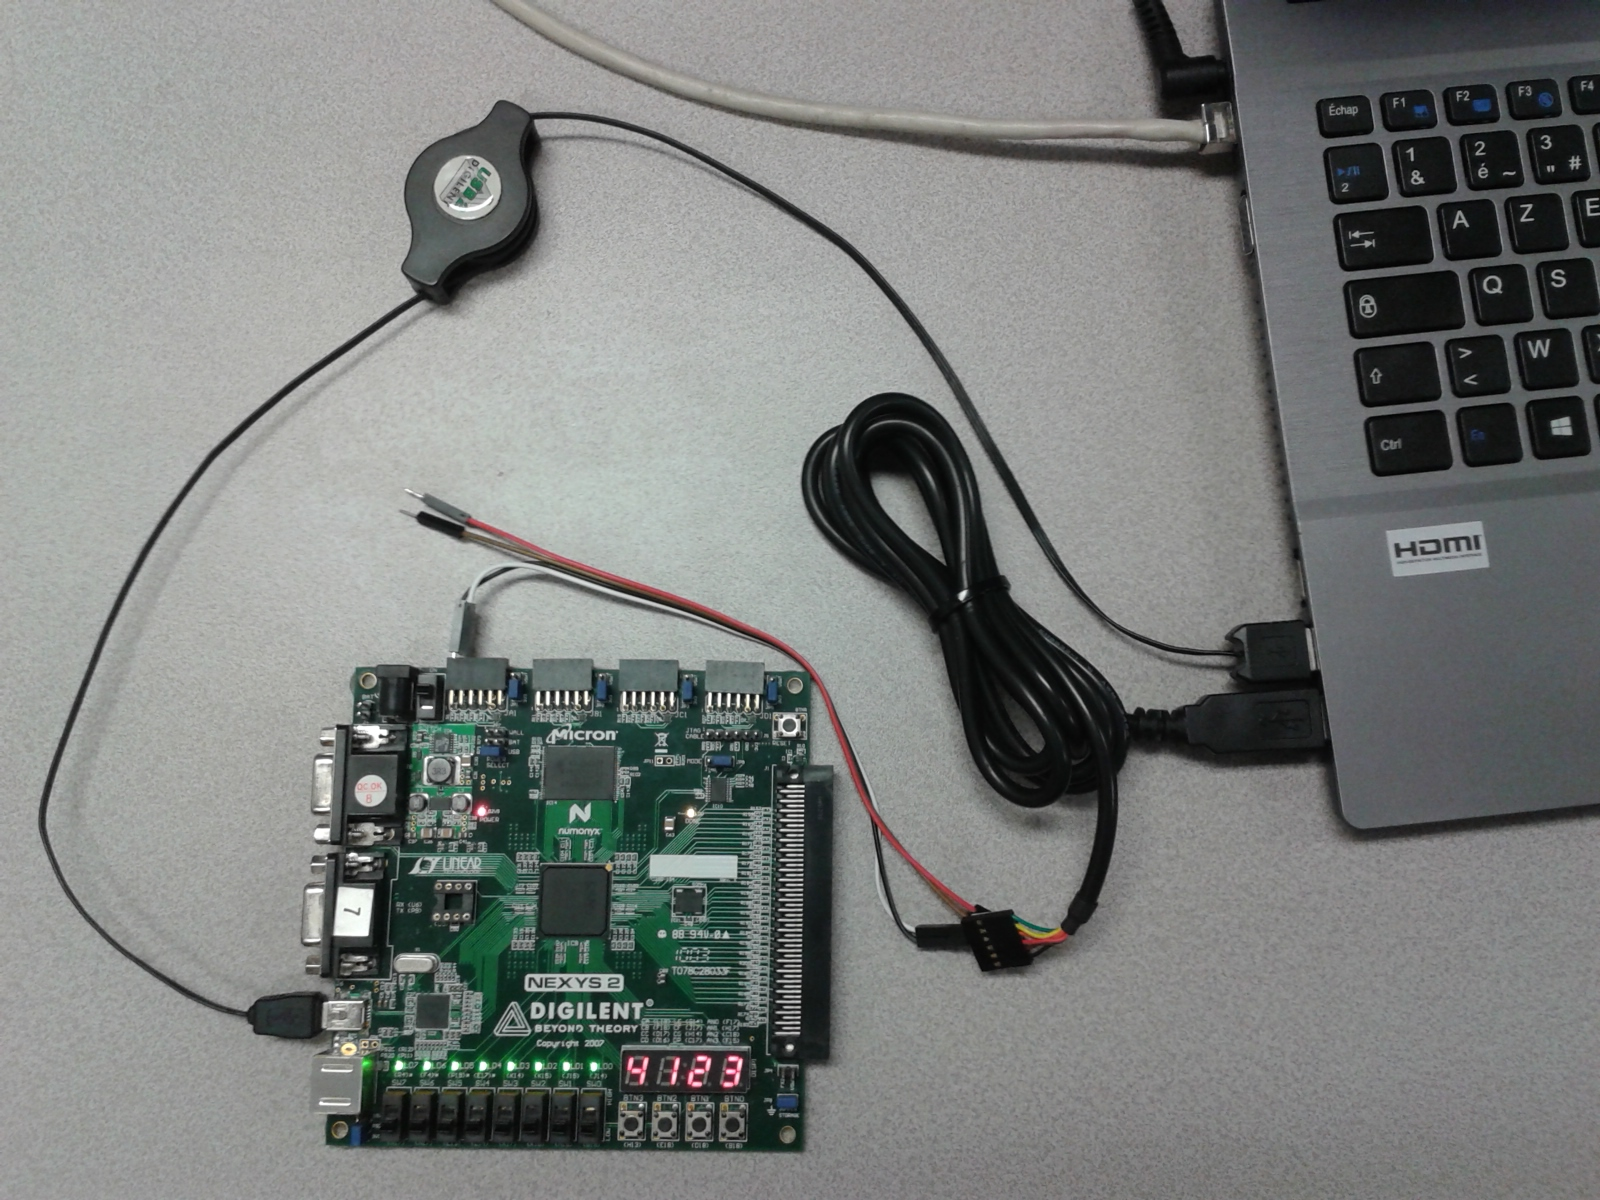
\includegraphics[width=0.8\textwidth]{./fig/Nexys2.jpg}
        \caption{A Nexys2 board}
      \end{figure}

    \section{Work required}
      The project is composed of three main tasks:
      \begin{itemize}
        \item improve the simple processor developed by students to add missing
          features;
        \item create a compiler for a \textit{C-like} language to the CRAPS
          assembly language;
        \item the operating kernel system itself.
      \end{itemize}

      All tools and source code produced will need to be documented for both
      teachers and students.

    \section{Available resources}
      Jean-Christophe Buisson initially lent us 2 boards. As this was not enough
      for the four of us to work efficiently, he lent us 4 more boards.
      He also gave us the sources of the tools he developed for his students so
      that we could adapt them for our needs.

      Our client got us a room in ENSEEIHT to work.

      \paragraph{}
      We also set up a \textit{git}\footnote{\textit{git} is distributed Version
      Control System (VCS).} repository to put all the sources and document we
      have produced during this project. This allowed us to efficiently work
      simultaneously on the same files and keep a history of all changes.
      We also set up a mailing list and a Jabber room\footnote{\textit{Jabber}
      is an instant messaging protocol.} to communicate with each other.

      We did all the work on our own personal computers.

  \chapter{Project management}
    The team is composed of four members:
    \begin{itemize}
      \item Korantin Auguste as \textit{developer}
      \item Maxime Arthaud as \textit{tester}
      \item Martin Carton as \textit{project leader}
      \item Étienne Lebrun as \textit{quality manager}
    \end{itemize}

    We were initially 5 but one of us had to leave the team for medical reasons
    at the beginning of the project.

    \section{Project supervision}
      We were affected to Xavier Mechin, quality control manager at Airbus
      Defence and Space to guide us in managing our project. Martin and Maxime
      met him the week before the project started (Korantin and Étienne were
      abroad). We decided to meet once a week. The date and order of the reunion
      is as follow:

      \begin{itemize}
        \item Week 0 (January 15th): presentations;
        \item Week 1 (January 22th): presentation of all members, presentation
          of the project management related work to do;
        \item Week 2 (January 28th): first review of the software development
          plan and specifications;
        \item Week 3 (February 4th): canceled due to the weather conditions;
        \item Week 4 (February 10th): review of the software development plan
          and specifications;
        \item Week 5 (February 18th): planning of the testing phase;
        \item Week 6 (February 25th): review of the test plan, planning of the
          final report and presentation;
        \item Week 7 (March 4th): TODO
        \item Week 8 (Martin 10th): TODO
      \end{itemize}

      During these meetings, Xavier explained us what documents we should
      produce for the management of the project and how to use them. Of course,
      as our project was short, we did not follow all Airbus practices but this
      showed us how do companies such as Airbus manage their project.

      \section{Risks management}
        Xavier asked us to list the risks of the project. This was difficult as
        the project is quite free but we were able to identify three risks.

        For each risk, the product $\text{probability} \times \text{gravity}$ is
        shown in the top-right cell. If the product is above 6, the risk is
        considered critical.

        \risk{3 \times 3 = 9}{
          A FPGA can be damaged, making any test impossible.
        }{
          This is likely to happen and very problematic but we have two FPGAs
          and the possibility to have more in case of problem.
        }{
          Actually, we have 6 FPGAs, the risk is considered closed.
        }

        \risk{2 \times 3 = 6}{
          We may not be able to integrate the RAM, leading to huge memory
          limitations that may make the project impossible.
        }{
          We are now able to use the RAM, the risk is closed.
        }{
          In case of memory limitations, we can try to optimize the size of the
          code we generate.
        }

        \risk{3 \times 1 = 3}{
          The communication between the board and the computer might be too slow.
        }{
          We will have to be very careful to send just what is needed.
        }{
          We would need to limit the communication. It is not necessarily a problem
          as this is just to show students how to implement a simple communication
          protocol.
        }

  \chapter{Specification phase}
    We planned a meeting with the client the first day of the project. He
    explained us what he wanted us to do and that the project was very flexible.
    His goal is to be able to make lab sessions for first-year students of
    ENSEEIHT. Thus, as long as he can show students how an operating system
    works the project will be a success.

    \section{Redaction of the technical specifications}
      Once we had determined the client's needs, we had to specify exactly what
      we had to do. This phase was difficult as the client was imprecise about
      what we had to do.

    \section{Technical choices}
      We choose to work as much as possible on GNU/Linux as this is our
      daily-use operating system and the operating system installed on most
      ENSEEIHT computers.
      However, the tools we needed were designed to work exclusively on
      Microsoft Windows. To get around this problem, we decided to use the
      Windows-specific tools in a virtual machine or adapt tools to GNU/Linux
      when possible.

      \subsection{Compiler}
        As we had to write a compiler but this is a very time-consuming task, we
        decided to reuse the compiler we had to write for a previous ENSEEIHT
        project. This compiler did not target the CRAPS machine, but we made it
        modular enough to able to easily add a CRAPS back-end.

        We considered for a moment to write a CRAPS back-end for \emph{LLVM}, a
        compiler infrastructure\cite{llvm}. This would have had the advantage to
        be able to used \emph{clang}, a real, complete and optimized
        \emph{C} compiler. But the work it would have required seemed to be too
        important as we did not know the \emph{LLVM} infrastructure and the
        infrastructure contains a lot of features we would not have used but
        would have had to support.

  \chapter{Implementation phase}
    \section{Interrupts}
      We first had to develop an interrupt system, to have the possibility of
      executing code when receiving data from the exterior.

      \subsection{Software interrupts}

    \section{Scheduler}
      The scheduler is the component that makes it possible to execute more than
      one task at a time: it will switch between all running task in a very fast
      way, giving the illusion that all processes runs at the same time.

      To have it work, we had to create a specific interrupt that will be
      triggered by a PWM that we define. This interrupt save the execution
      context (all the registers of the processor) and restore the one of the
      next process to execute.

      To do that, we also have a data structure containing the list of the
      processes. First, it was simply a list that was redimensionned when we
      added/deleted processes.  However, we ended up changing it to a list of a
      fixed size, containing either pointer to processes stacks, or null values.
      This allowed the processes to have a fixed ID that will not change during
      their life.  With that knowledge, the process management was made more
      easy, and it was also possible to annotate memory zones with the
      associated process ID, leading to clean freeing of all the memory
      allocated by processes when they were terminated.

    \section{Serial Port}
      Is slow, but works.

    \section{Memory management}
      For the dynamic loading of processes to work, we needed to be able to
      allocate memory zones (for processes stacks). It was also really important
      to have the possibility for processes to allocate the memory they need.

      So, we had to create the equivalent of malloc/realloc/free. We did a very
      simple implementation: starting from a base pointer, we store block of
      memory. These blocks starts with a header indicating their size, the
      process ID that allocated them (and a byte to tell if the block is free or
      not).

      The size of each block is a power of two. So when we allocate a block, we
      will try to see if there is a free block of the good size. If there is
      not, we will create a new block at the end of the block list.
      So, we don't merge or split blocks, and will waste memory. But it keeps
      the implementation simple, and the block are reused a lot, in general.

    \section{Compiler}
      Needed to support a language very close to C. Generate CRAPS Assembly.

      \subsection{Optimizations}
        All the optimizations made by the compiler.

    \section{Dynamic loading}
      We were able to directly upload code\dots

    \section{Final result}
      A lot of test tasks.

      A shell communicating via the serial.
      Add screens of the shell (real screens of a terminal), and list commands.

  \chapter{Validation phase}

    \section{Tests}

    \section{Limitations}

  \chapter{Conclusion}

  \addcontentsline{toc}{chapter}{Bibliography}
  \begin{thebibliography}{9}
    \bibitem{buisson}
      Jean-Christophe Buisson,
      \emph{Introduction à l'architecture des ordinateurs},
      Chapitre VII.\ CRAPS~: guide du programmeur.

      \mbox{\url{http://diabeto.enseeiht.fr/download/archi/cours/book2_4.4.pdf}}

    \bibitem{nexys2}
      \emph{Digilent Nexys2 Board, Reference Manual},
      Revision: July 11, 2011.

      \mbox{\url{http://www.digilentinc.com/data/products/nexys2/nexys2_rm.pdf}}

    \bibitem{llvm}
      \emph{Writing an LLVM Backend}

      \mbox{\url{http://llvm.org/docs/WritingAnLLVMBackend.html}}
  \end{thebibliography}

  \addcontentsline{toc}{chapter}{Annexes}
  \chapter*{Annexes}
    \newgeometry{top=1cm,bottom=1cm}
    \thispagestyle{empty}
    \begin{figure}
      \centering
      \includegraphics[
        angle=90,
        width=\linewidth,
        height=\textheight
      ]{Gantt.pdf}
      \label{fig:gantt}
    \end{figure}
    \clearpage
    \restoregeometry
\end{document}
